\section{The Large Hadron Collider}
The Large Hadron Collider~\cite{Evans:2008zzb} is the world's 
largest and most powerful particle accelerator. 
It started operation in 2008 and retains its crucial role in the many 
accelerators in the world.
The collider is located in a ring tunnel of 
circumference 26.7 km, which lies beneath the 
French-Swiss border near Geneva, with superconducting magnets 
along the tunnel to keep the particle beam in direction
and a large number of accelerating structures to boost the 
beam to the desired energy.
Inside the tunnel, \textit{bunches} of up to $1.15 \times 10^{11}$ protons
travelling at close to the speed of light in opposite direction 
are collided 40~million times per second at four cross points,
around which are positioned four main detetors: 
ATLAS (A Toroidal LHC ApparatuS)~\cite{PERF-2007-01}, 
CMS~\cite{CMS-2008xjf} (Compact Muon Solenoid), ALICE (A Large Ion Collider Experiment) 
\cite{ALICE-2008ngc} and LHCb (b stands for beauty)~\cite{LHCb-2008vvz}.

% All the controls for the accelerator, its services and technical infrastructure 
% are located at the CERN Control Centre. 
% From here, the beams inside the LHC are made to collide 
% at four locations around the accelerator ring, 
% corresponding to the positions of four particle 
% detectors.

% two beams of particles travelling at close 
% to the speed of light 
% in opposite direction are made to collide. 


% Thousands of magnets are used to direct the beams 
% along the beam pipe, either to bend the beams or
% to focus them. The particles are so small that 
% making them collide is akin to firing two needles 
% 10 kilometers apart and getting them to meet halfway. 
	
\subsection{The LHC Accelerator Complex}

The proton beams colliding in the LHC are designed to carry energy 
of the order of a few TeV. To reach such high energy, a series of 
acceleration is required for the beams before entering the LHC ring. 
The protons are supplied by the injector chain Linac 2 — Proton Synchrotron 
Booster (PSB) — Proton Synchrotron (PS) — Super Proton Synchrotron (SPS), 
as shown in Figure~\ref{fig:accelerator_complex}.

\begin{figure}[bht]
	\begin{centering}	
	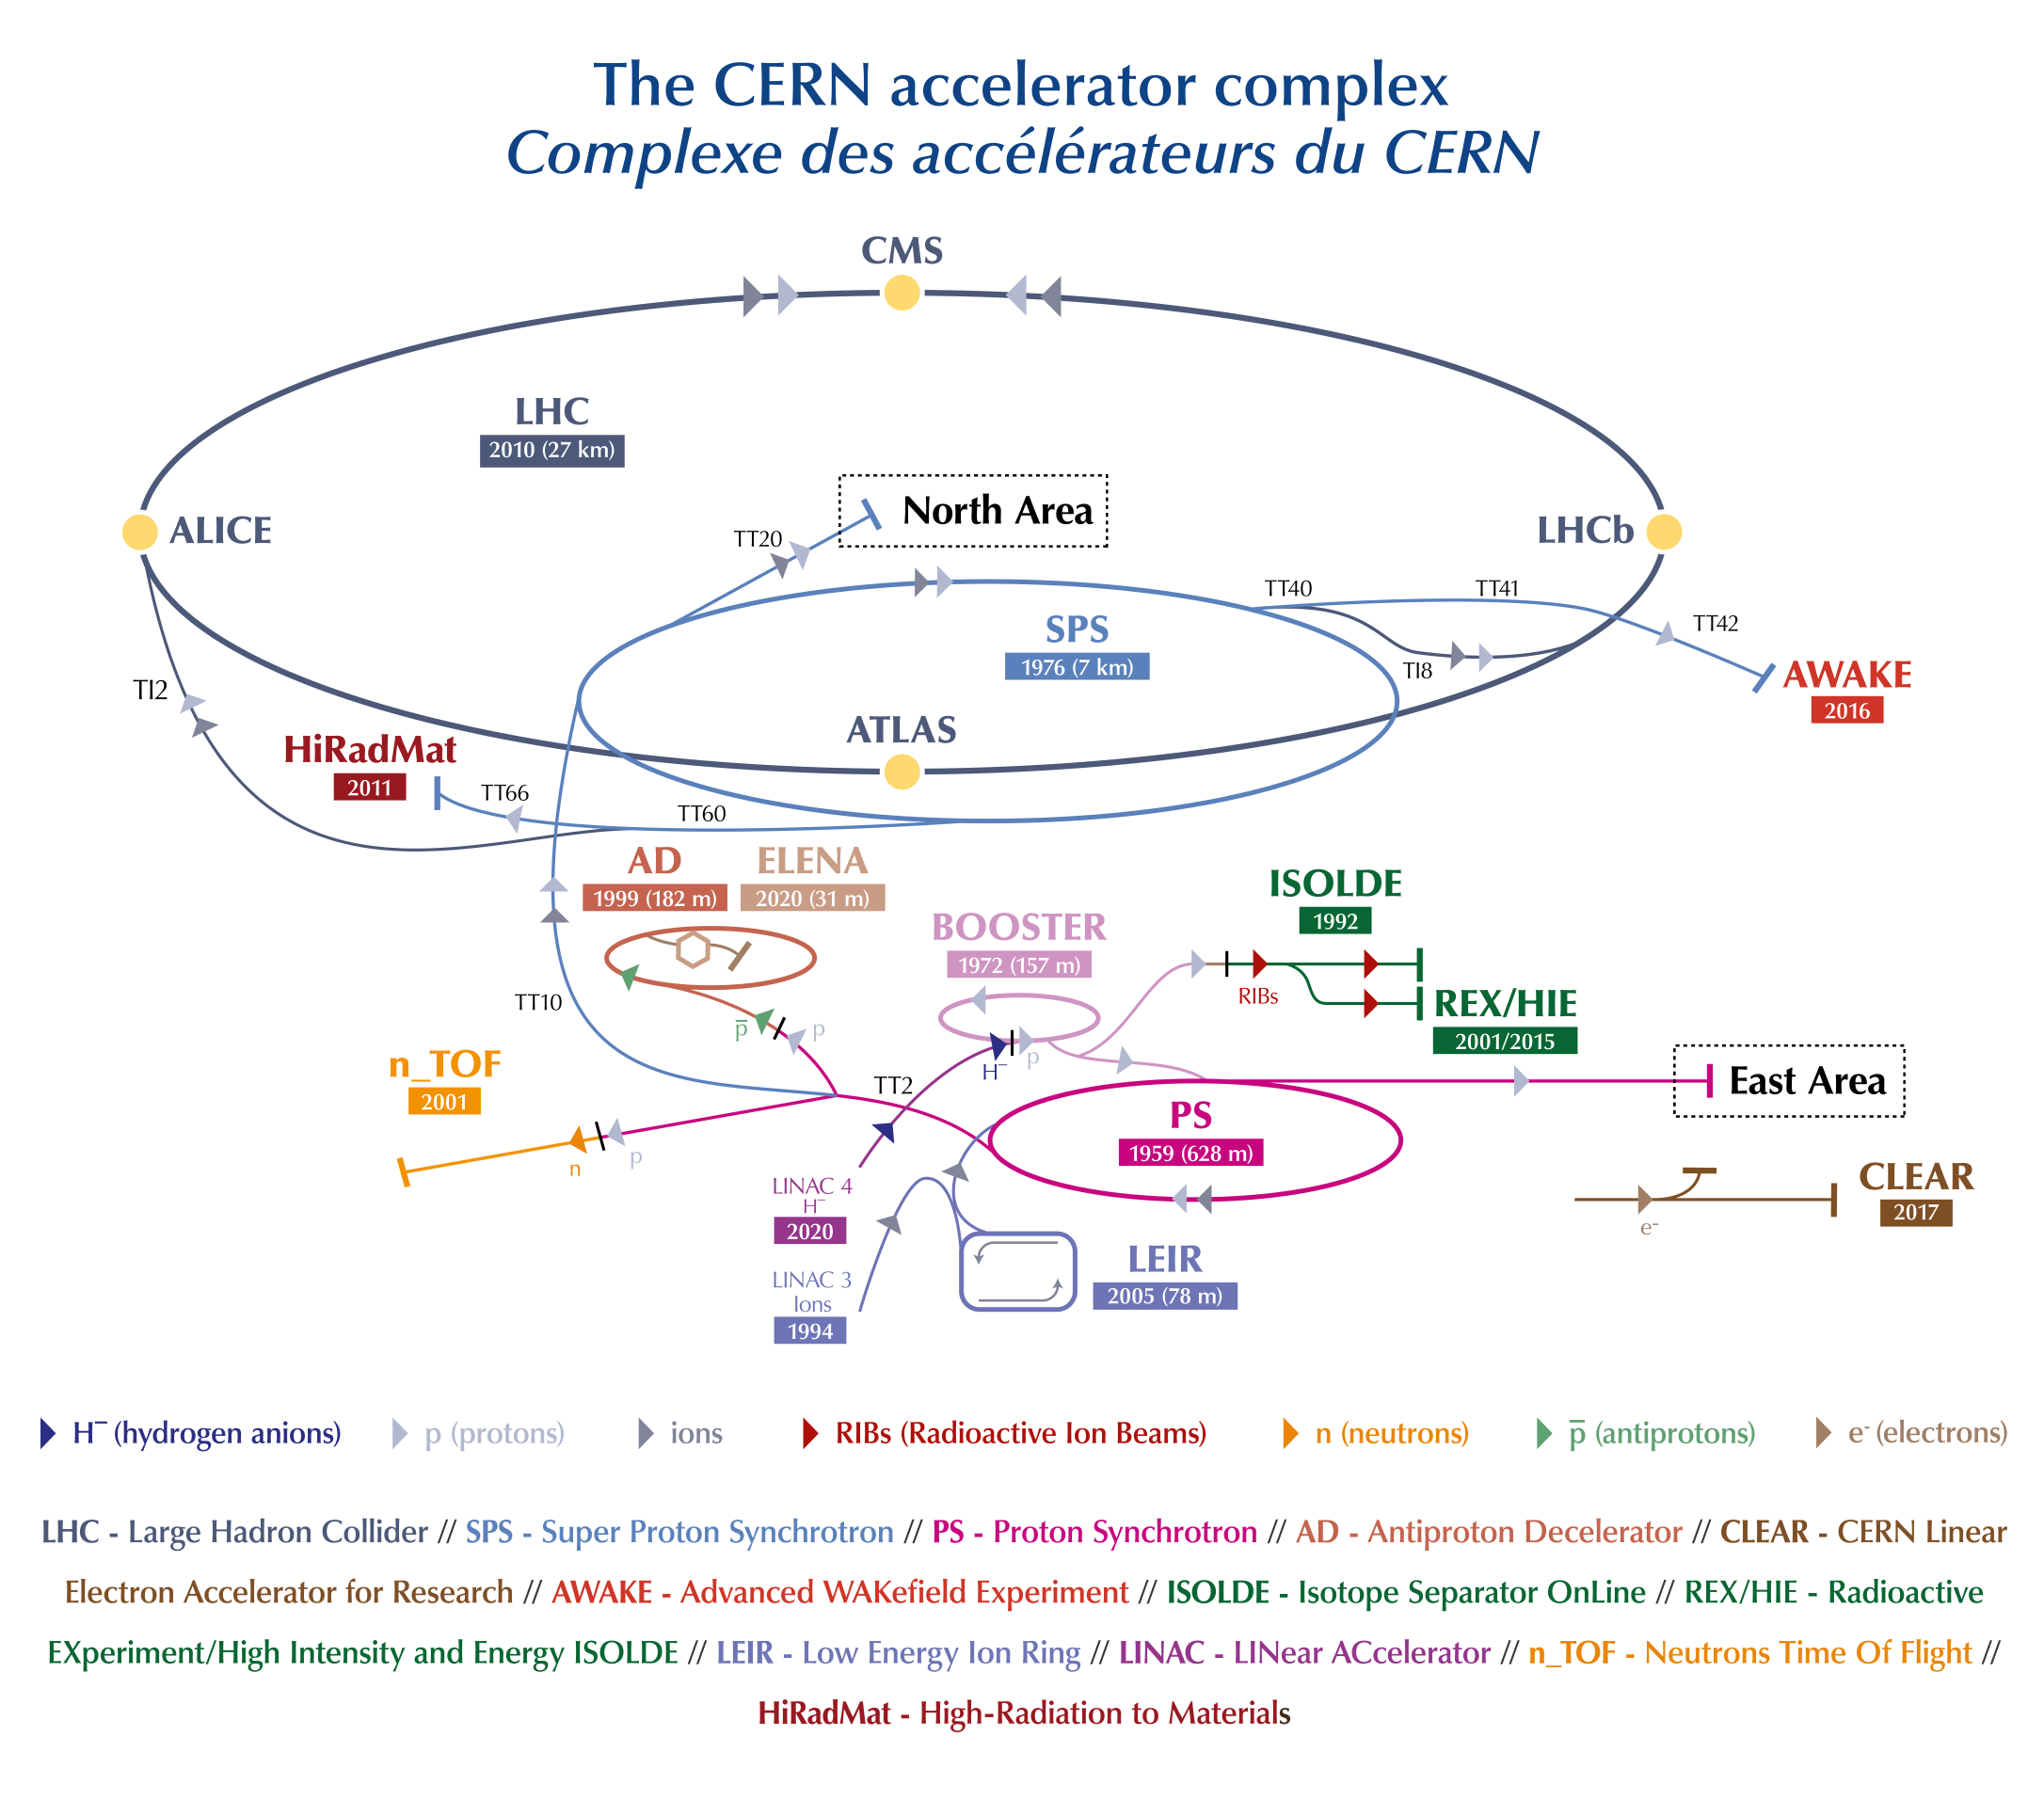
\includegraphics[width=.9\textwidth]{Detector/plots/accelerator_complex_smaller.png}
	\caption{The LHC is the last ring (dark blue line) in a complex chain of 
	particle accelerators. The smaller machines are used in a chain to help boost 
	the particles to their final energies and provide beams to a whole set of smaller experiments.
		}
	\label{fig:accelerator_complex}
	\end{centering}
\end{figure}

The protons are produced by stripping off the electrons from hydrogen gas
in an electric field. Linac 2, the first accelerator in the chain, 
is a linear accelerator which accelerates the protons to an energy of 50~MeV. 
They then enter the PSB, which accelerates the protons to 1.4~GeV, followed by 
the PS, where they reach 25~GeV. The series of radio frequency cavities in 
the PS splits the beam into discrete bunches of protons of 25 ns spacing. 
These bunches are then accelerated to 450~GeV in the SPS, from which they 
are finally injected into the beam pipes of the LHC. 
Each proton beam contains 2808 bunches, arranged in ``trains''
with 72 bunches each ``carriage'' of a gap of around 320 ns between each carriage. 
The beams are required to have well defined transverse and longitudinal emittance. 

The beam pipes are kept at ultra-high vacuum, a vacuum thinner than 
interstellar void, matianed for 24 km of low-temperature section and 3 km 
of room-temperature section. For the low temperature section, the vacuum is 
achieved by pumping in $9000$ m$^3$ of cryogenic gas, which later will be 
condensed and adhered to the surface of the beampipe. 
For the room temperature section, the vacuum 
is achieved by use of non-evaporable getter (NEG) that absorbs residue 
gas particles when heated. More residue is absorbed by an ion pumper. 

The beam pipes are installed in the existing tunnel that was constructed 
between 1984 and 1989 for the Large Electron-Positron Collider (LEP)~\cite{Myers:1991ym}, 
which lies between 45~m and 170~m below the surface on a plane inclined at 1.4\% sloping 
towards the Léman lake.
% Approximately 90\% of its length is in molasse rock, which has excellent 
% characteristics for this application, and 10\% is in limestone under the Jura mountain. 
% There are two transfer tunnels, each approxi-mately 2.5 km in length, linking the 
% LHC to the CERN accelerator complex that acts as injector. 
% These two beams are kept in separate beam pipes,
% cooled to $-271.3^\circ$C ($1.9$ K) with liquid 
% helium distributed by dedicated system, 
%  and ultra-high vacuum, 
There are advantages and disadvantages for a proton-proton collider,
compared to the electron-positron collider like LEP or proton-anti-proton collider.
% The proton-proton collider has advantages 
% and disadvantages compared 
For the LHC, two rings are needed to accommodate the two counter-rotating beams, 
unlike particle-antiparticle colliders that can have both beams sharing the same 
phase space in a single ring, and therefore sharing the same magnets, same radio 
frequency cavities, etc. However, LHC is able to achieve very high collision energy
which is not possible using electron-positron colliders, neither linear nor circular ones.
This is due to the fact that in a circular electron collider, synchrotron radiation lost is 
proportional to the Lorentz factor $\gamma = E/m$ to the power of four, where $E$ and $m$ are
the energy and mass of the particle, respectively. Since electrons are about
2000 times lighter than protons, synchrotron radiation lost is at the order of $10^{13}$
faster for electrons than for protons. For linear electron-positron collider, an extremely long
acceleration section is required with current technologies, which makes it an impractical option.
As for the proton-anti-proton collider, it would not be possible to achieve such 
high luminosity using anti-proton beams, since it is much more difficult 
to produce anti-protons than to produce protons. In addition, at high energies
the proton anti-proton collider starts losing one of its advantages of having higher cross section, 
which is due to the quark sea and anti-quarks in protons become more ``visible'' at high
energies (more details in the parton model section).
% In principle, since the mass of the proton is much larger than 
% the mass of the electron, the
% synchrotron radiation for the losses will be much smaller, and 
% the long straight sections designed to compensate the losses 
% (as designed for the LEP) can be reduced. 
% However these sections are kept 
% as the LEP has as a cost-effective solution, which avoids  
% re-excavating the tunnel. 
% The tunnel in the arcs has a finished internal diameter of 3.7~m. 

As explained above, two separate rings are required to accomodate the two beam pipes, while
the internal diameter of the tunnel is only about 3.8~m. It's technically challenging to 
install them in such small space. LHC therefore adopted the twin-bore magnet design~\cite{rossi2003lhc}, 
as shown in Figure~\ref{fig:double-bore-magnet}. It was first proposed by John Blewett at the Brookhaven 
laboratory in 1971 due to cost considerations~\cite{Blewett:1971zzb}, but in the case 
of the LHC the overriding reason for adopting this solution	is the lack of space in the tunnel. 
\begin{figure}[bht]
	\begin{centering}	
	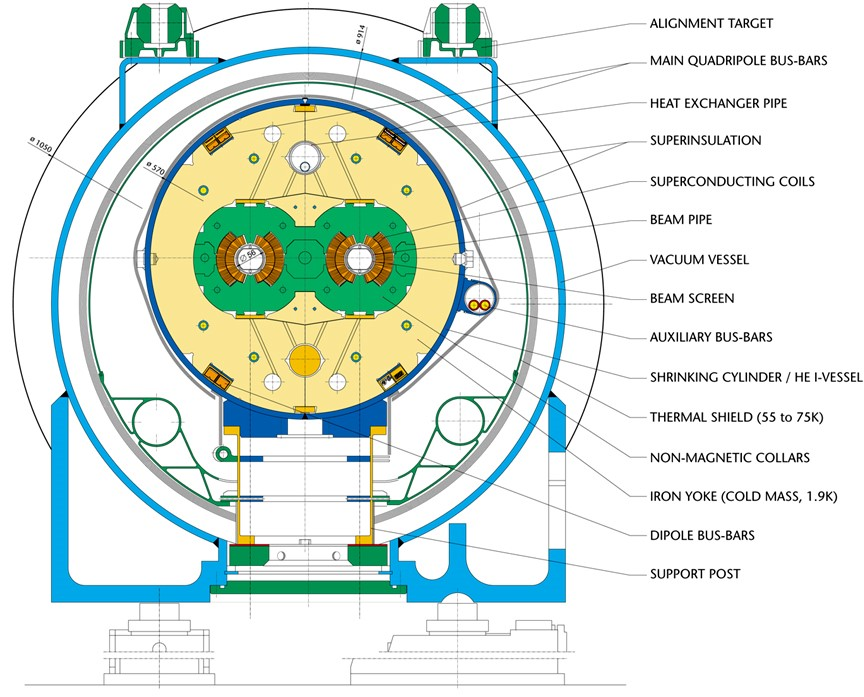
\includegraphics[width=.7\textwidth]{Detector/plots/LHC-double-bore-magnet.jpg}
	\caption{ Double-bore magnet configuration of the LHC 
	superconducting magnets~\cite{rossi2003lhc}.}
	\label{fig:double-bore-magnet}
	\end{centering}
\end{figure}

\subsection{Luminosity and pileup}
\label{sec:LHC:pileup}
% The aim of the LHC is to reveal the physics beyond
% the Standard Model with centre of mass collision energies of up to 14 TeV.
Luminosity is an important measure of a collider's performance.
It comes closely to the number of events generated per second, given by:
\[
	N = \mathcal{L}\sigma,
\]
where $\sigma$ is the scattering cross section 
for the event under study and $\mathcal{L}$ is the machine luminosity. 
For the cross-section, it is more common to use barn as the unit, 
where 1b~=~10$^{-28}$~m$^2$~=~10$^{-24}$~cm$^2$, 
since particle interactions usually have very small cross-sections. 
The machine luminosity depends on the beam parameters 
and can be written for a Gaussian beam distribution as:
\[
	\mathcal{L} = \frac{N_b^2 n_b f_{rev} \gamma_r}{4\pi \epsilon_n \beta*} F,
\]
where $N_b$~refers to the number of protons per bunch,
$n_b$~is number of bunches per beam,
$f_{rev}$~is the revolution frequency, 
$\gamma_r$~is the relativistic gamma factor, 
$\epsilon_r$~is the normalised transverse beam emittance, 
$\beta*$~is the beta function at the collision point which
describes the size of the beam, 
and	$F$ refers to the geometric luminosity reduction factor due to the 
crossing angle at the interaction point. 
While the instantaneous luminosity measures the rate of collisions (per unit cross-section), 
the total number of collisions (per unit cross-section) is measured by the integrated luminosity L, 
given by:
\[
	L = \int \mathcal{L} dt,
\]
which is the integral of the instantaneous luminosity over time.

The two general purpose experiments, ATLAS and CMS are
both aiming at a peak luminosity of $\mathcal{L}$ = $10^{34}$ cm$^2$s$^{-1}$ for proton proton collision,
which corresponds to about one billion $pp$ collisions per second. 
The instantaneous luminosity was much improved at real-time operations reaching about 
twice the nominal (from 2015 to 2018) thanks to the effort of the LHC experts. 

Another important parameter for the LHC experiments is the pileup, 
which is a measure of the number of inelastic $pp$ interactions that occur per bunch crossing. 
Higher pileup gives more luminosity (for a fixed number of bunches) 
but makes physics analysis more difficult due to the signals in the detector 
from the additional interactions. The distribution of the recorded luminosity over
the pileup is shown in Figure~\ref{fig:Run2_pileup} for operations from 2015 to 2018 (Run 2), 
where the <$\mu$> stands for the mean number of interactions per bunch crossing.
There are two main sources of pileup: in-time pileup and out-of-time pileup.
The former refers to the additional proton-proton collisions occuring in
the same bunch-crossing as the collision of interest. 
The later refers to the additional proton-proton collisions occuring
in bunch-crossings just before and after the collision of interest. 
% The out-of-time pileup is a challenge for the detector subsystems that 
% have sensitivity windows longer than
% 25 ns, the interval between bunch crossings.
%  It's a challenging task for the 
% trigger and reconstruction algorithms to achieve robustness under such high pileup 
% condition.
\begin{figure}[bht]
	\begin{centering}	
	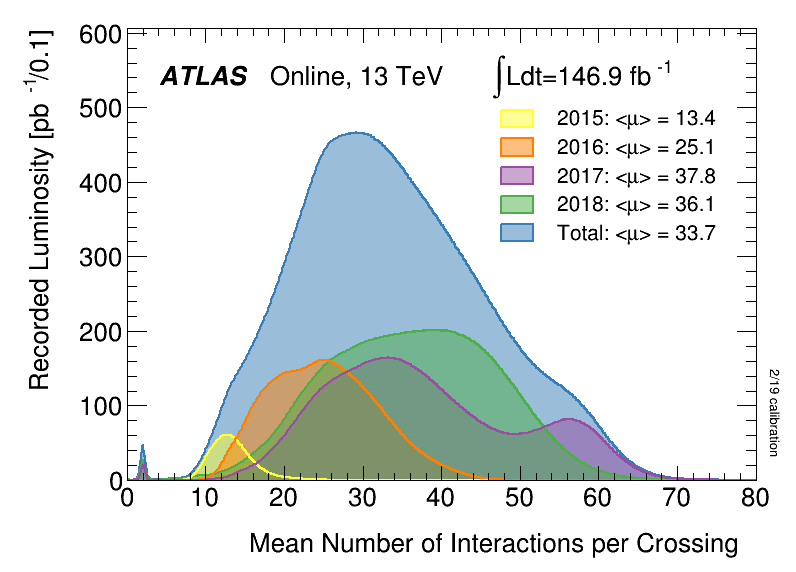
\includegraphics[width=.6\textwidth]{Detector/plots/Run2_pileup.png}
	\caption{Shown is the luminosity-weighted distribution of the mean number of 
	interactions per crossing for the data collected by the ATLAS from 2015 to 2018. 
	All data recorded by ATLAS during stable beams is shown, and the integrated luminosity and 
	the mean $\mu$ value are given in the figure. 
		}
	\label{fig:Run2_pileup}
	\end{centering}
\end{figure}

\subsection{Operation schedule}
\label{sec:Operation schedule}
The LHC operation and shutdown schedule is shown 
% in Figure~\ref{fig:LHC-longterm-schedule}
in Figure~\ref{fig:LHC-schedule-lumi}.
Following the downtime after an incident in one of the main dipole circuits 
during the first commissioning in 2008~\cite{lebrun2009report},
the operation restarted at lower beam energy to minimise the risk. 
Therefore, the first proton run (2010-2013)~\cite{alemany2013operation} was
carried out at 3.5–4 TeV per beam (centre of mass energy 7-8 TeV). 
Furthermore, a bunch spacing of 50 ns was used instead of the nominal 25 ns,
% This implied fewer bunches with larger intensity and hence a 
with peak luminosity of 0.8 $\times$ 10$^{34}$ cm$^{-2}$s$^{-1}$, 
% still smaller than
% the nominal 10$^{34}$ cm$^{-2}$s$^{-1}$ luminosity) 
and pileup larger than nominal. 
% \begin{figure}[bht]
% 	\begin{centering}	
% 	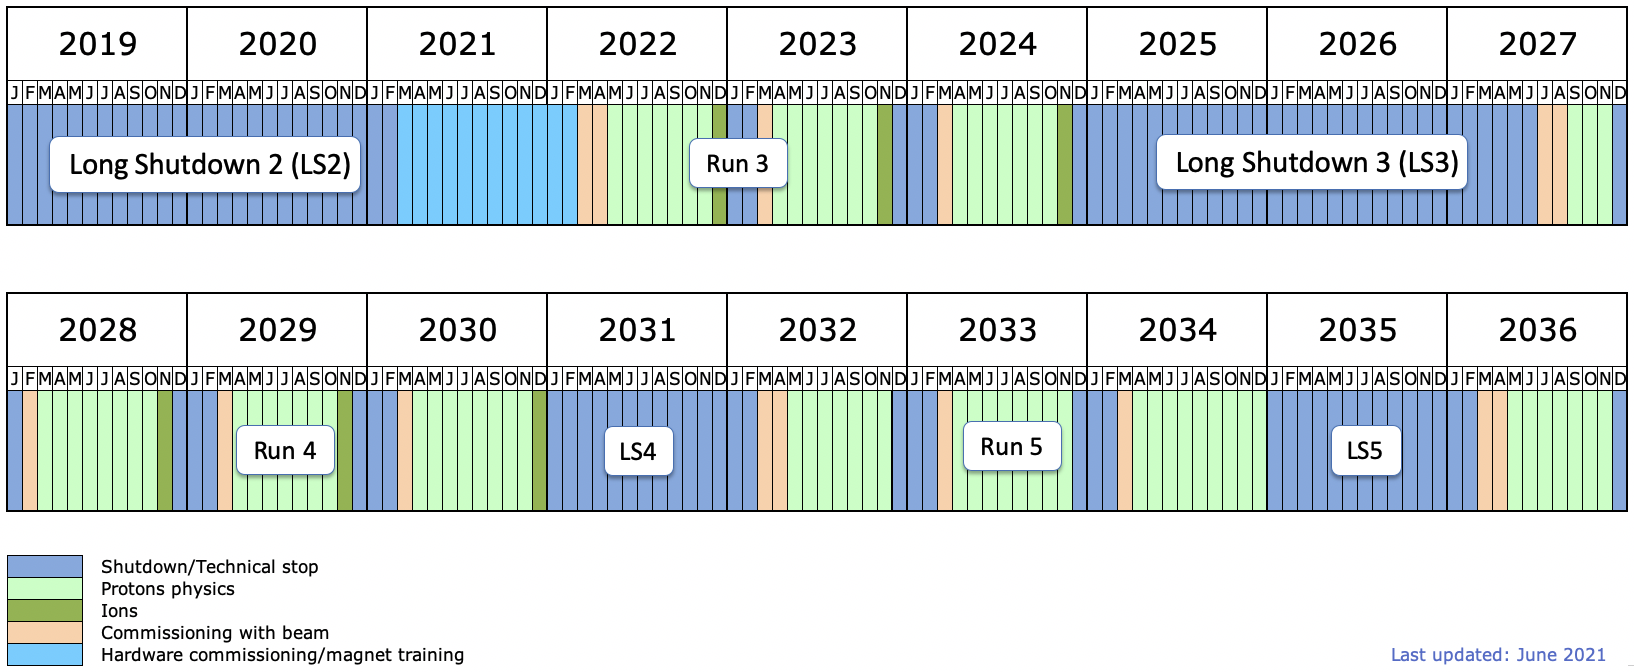
\includegraphics[width=.9\textwidth]{Detector/plots/LHC-longterm-schedule.png}
% 	\caption{Longer term LHC operation schedule.% [source: https://lhc-commissioning.web.cern.ch/schedule/LHC-long-term.htm]
% 		}
% 	\label{fig:LHC-longterm-schedule}
% 	\end{centering}
% \end{figure}

\begin{figure}[bht]
	\begin{centering}
	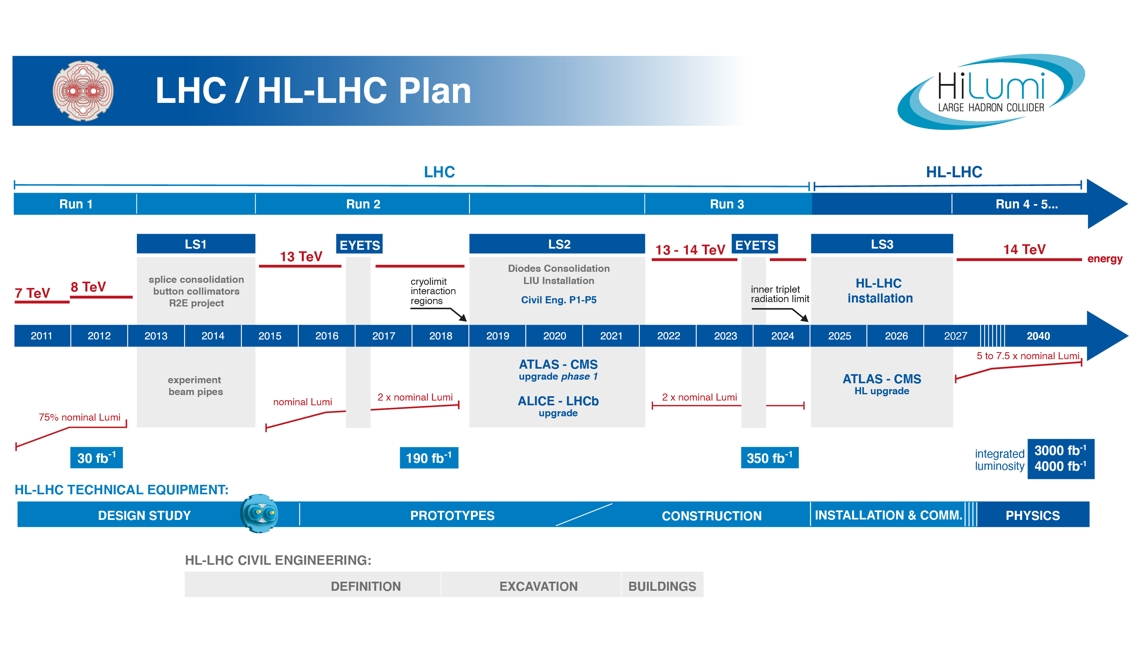
\includegraphics[width=.95\textwidth]{Detector/plots/LHC-schedule-lumi.jpg}
	\caption{LHC operation schedule and luminosity targets.  %[source:project HL-LHC, https://project-hl-lhc-industry.web.cern.ch/content/project-schedule ]
		}
	\label{fig:LHC-schedule-lumi}
	\end{centering}
\end{figure}
In Run 1, the LHC delivered about 30~\fb\ of proton data and important physics results,
most notably the discovery of the Higgs boson~\cite{HIGG-2012-27,HIGG-2012-28}.
Run 1 was followed by a long shutdown (LS1, 2013–2014)
with a large number of consolidation and upgrade activities~\cite{bordry2013first}. 	
The bus-bar splices between the superconducting magnets were improved, 
in order to make sure that the LHC could operate at higher energy 
without risk of repeating the 2008 incident. 

\begin{figure}[bht]
	\begin{centering}	
	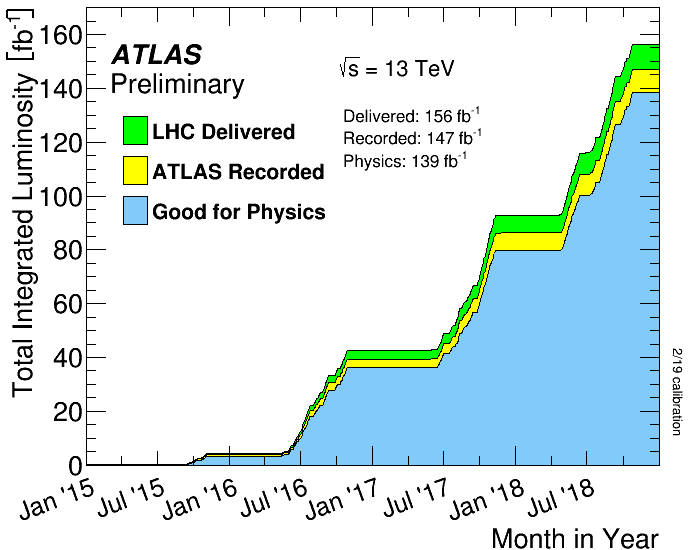
\includegraphics[width=.6\textwidth]{Detector/plots/Run2_lumi.png}
	\caption{Cumulative luminosity versus time delivered to 
	ATLAS (green), recorded by ATLAS (yellow), and certified to be 
	good quality data (blue) during stable beams for $pp$ collisions 
	at 13 TeV centre-of-mass energy in Run 2. 
		}
	\label{fig:Run2_lumi}
	\end{centering}
\end{figure}

Run 2 (2016-2018) was carried out
at 6.5 TeV per beam (center of mass energy 13 TeV)~\cite{LHC-Run2-Operation}. 
As shown in Figure~\ref{fig:Run2_lumi}, out of the 156~\fb\ 
of data LHC has delivered at 13 TeV centre of mass energy, the ATLAS detector has recorded 
147~\fb\ and \lumi\ of data is certified to be good quality data.
The 156~\fb\ data accounts for the luminosity delivered from the start of 
stable beams until the LHC requests ATLAS to put the detector in a 
safe standby mode to allow a beam dump or beam studies. 
The recorded luminosity is slightly smaller than the delivered luminosity, due 
to the inefficiency of the Data Acquisition and the so called ``warm start'': 
when the stable beam flag is raised, 
the tracking detectors undergo a ramp of the high-voltage and, 
for the pixel system, turning on the pre-amplifiers. 
More details of the ATLAS detector can be found in the following sections. 
The recorded data is checked carefully to exclude possible hardware or software  issues. 
This is achieved by monitoring detector-level quantities 
and reconstructed collision event characteristics at key stages of the data processing chain.
This procedure led to high efficiency of good quality data: 95.6\%~\cite{aad2020atlas}.	

In this thesis the \lumi\ data recorded by the ATLAS detector of Run 2 is used.
The nominal bunch spacing of 25 ns was used, with slightly less bunches (2500) per beam.
The LHC experts have continually improved the running scenario to increase the luminosity,
and during Run 2 the luminosity surpassed the designed luminosity by a factor of 2. 
As well as improving the instantaneous luminosity, the availability of the machine
was dramatically improved during Run 2 which is an important factor enabling the high efficiency 
of good quality data as mentioned above.
During Run 2, the machine was providing physics collisions during 50\% of 
the allocated physics time, which is very impressive for a super conducting collider. 

The operation of CERN’s accelerators is subject to scheduled shutdowns 
to allow important repair and upgrade work to take place. 
The present shutdown, LS2, is devoted to preparations for Run 3 of the LHC, 
which will have an integrated luminosity equal to the two previous runs combined, 
and for the High-Luminosity LHC (HL-LHC), 
the successor to the LHC, which will begin operation at the end of 2027,
and eventually generate 10 times the integrated luminosity of
all Run 1, 2 and 3 combined!

The LS2 schedule has had to be modified due to the COVID-19 pandemic, 
which the new schedule anticipates that the first test beams will 
circulate in the LHC 
at the end of September 2021, four months later than the date 
planned before the COVID-19 crisis, 
to give the LHC’s main experiments – ATLAS, CMS, ALICE and LHCb – 
time to prepare their own upgrade. 
Run 3 of the LHC will begin at the start of March 2022.
% No changes have been made to the schedule beyond 2022.
The third long shutdown (LS3) will begin at the 
start of 2025 and end in mid-2027. 
This is when the equipment for the HL-LHC and 
its experiments will be installed. 
